% SC3270 --- Chapter 6: Weakest Preconditions - Dijkstra's Calculus (0->100 ground-up)
\chapter{Weakest Preconditions: Reasoning Backwards}
\label{ch:wp}

\begin{quote}
\emph{``Program and proof develop hand in hand.''} Instead of guessing a precondition and checking forwards, calculate backwards: from the desired post, what must have been true before?
\end{quote}

\noindent\fbox{\parbox{\dimexpr\linewidth-2\fboxsep-2\fboxrule}{%
\textbf{From zero: no wp experience assumed.} We define weakest preconditions from scratch, show how substitution makes assignment trivial, and build the calculus for sequence, conditional and loops. Pictures motivate each rule before formalism.}}
\vspace{0.4em}

\section*{Learning Outcomes}
After this chapter you will be able to:
\begin{enumerate}[label=(L\arabic*)]
    \item define $\text{wp}(C,Q)$ and explain ``weakest'' as the largest pre-set guaranteeing $Q$;
    \item compute $\text{wp}$ for assignment, sequence, and conditional by substitution and case split;
    \item relate $\text{wp}$ to Hoare triples: $\{P\}\,C\,\{Q\}$ iff $P\Rightarrow\text{wp}(C,Q)$;
    \item approximate $\text{wp}$ for loops via invariants and iterate;
    \item use $\text{wp}$ to generate VCs and connect to symbolic execution.
\end{enumerate}

% ============================================================
\section{Reasoning Backwards}
\label{sec:backwards}
\paragraph{Intuition.} Forward reasoning says: ``I know $P$, I run $C$, what can I conclude?'' Backward reasoning says: ``I want $Q$ afterwards, what must I ensure before?'' The second is more useful for verification: the post is the goal; the pre is the obligation you must discharge at the call site.

If $\{P\}\,C\,\{Q\}$ holds, any stronger $P'$ also works. The \emph{weakest} precondition is the \emph{most permissive} $P$ that still guarantees $Q$—the largest set of states from which $C$ must land in $Q$ (if it terminates). Every other correct $P$ implies it.

\begin{definition}[Weakest precondition]
$\text{wp}(C,Q)$ is the weakest assertion such that $\{\text{wp}(C,Q)\}\,C\,\{Q\}$ holds and for any $P$, $\{P\}\,C\,\{Q\}$ iff $P\Rightarrow \text{wp}(C,Q)$. Dual: $\text{sp}(P,C)$ is the strongest postcondition with $\{P\}\,C\,\{\text{sp}(P,C)\}$ and $\text{sp}(P,C)\Rightarrow Q$ for any valid $Q$.
\end{definition}

\begin{figure}[h]\centering
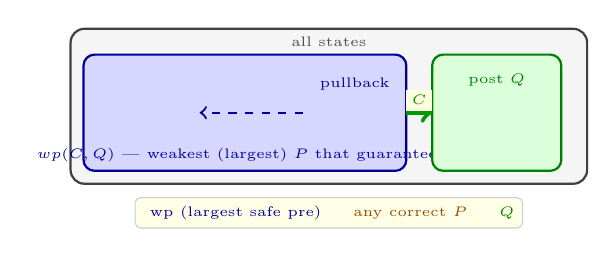
\begin{tikzpicture}[scale=0.82,font=\scriptsize]
\draw[fill=gray!08,draw=gray!50!black,thick,rounded corners=5pt] (0,0) rectangle (8.0,2.4);
\node[font=\tiny,gray!60!black] at (4.0,2.20) {all states};
\draw[fill=orange!12,draw=orange!60!black,thick,rounded corners=4pt] (0.4,0.30) rectangle (3.6,1.90);
\node[font=\tiny,orange!60!black,align=center] at (2.0,1.60) {some $P$\\stronger};
\draw[fill=blue!16,draw=blue!60!black,thick,rounded corners=4pt] (0.2,0.20) rectangle (5.2,2.00);
\node[font=\tiny,blue!60!black,align=center] at (2.80,0.45) {$\text{wp}(C,Q)$ --- weakest (largest) $P$ that guarantees $Q$};
\draw[fill=green!14,draw=green!50!black,thick,rounded corners=4pt] (5.6,0.20) rectangle (7.6,2.00);
\node[font=\tiny,green!50!black,align=center] at (6.60,1.60) {post $Q$};
\draw[->,ultra thick,green!60!black] (5.2,1.10) -- (5.6,1.10) node[midway,above,font=\tiny,fill=yellow!12,inner sep=2pt] {$C$};
\draw[->,thick,blue!60!black,dashed] (3.6,1.10) -- (2.0,1.10);
\node[font=\tiny,blue!60!black] at (4.4,1.55) {pullback};
\node[font=\tiny,align=left,fill=yellow!10,draw=gray!40,rounded corners=2pt,inner sep=3pt] at (4.0,-0.45) {\textcolor{blue!60!black}{$\blacksquare$ wp (largest safe pre)} \quad \textcolor{orange!60!black}{$\blacksquare$ any correct $P$} \quad \textcolor{green!50!black}{$\blacksquare$ $Q$}};
\end{tikzpicture}
\caption{$\text{wp}(C,Q)$ as the pullback of $Q$ through $C$: the largest pre-set that must land in $Q$. Any correct $P$ sits inside $\text{wp}$.}
\label{fig:wp-pullback}
\end{figure}

So to check $\{P\}\,C\,\{Q\}$, compute $\text{wp}(C,Q)$ and test the single implication $P\Rightarrow\text{wp}(C,Q)$—no need to reason about $C$ again. This reduces verification to logic.

% ============================================================
\section{Calculus: wp by Syntax}
\label{sec:wp-calculus}
\paragraph{Intuition.} Each command transforms the desired post backwards into a pre. The rules are:

\textbf{Skip:} $\text{wp}(\texttt{skip},Q)=Q$—nothing changes.

\textbf{Assignment:} $\text{wp}(x:=e, Q)=Q[x\mapsto e]$—substitute $e$ for $x$ in $Q$. Example: $\text{wp}(x:=x+1,\;x>5) \equiv (x+1>5)\equiv x>4$.

\textbf{Sequence:} $\text{wp}(C_1;C_2,Q)=\text{wp}(C_1,\text{wp}(C_2,Q))$—work backwards, inside out.

\textbf{Conditional:} $\text{wp}(\texttt{if }B\texttt{ then }C_1\texttt{ else }C_2, Q)= (B\Rightarrow\text{wp}(C_1,Q))\land(\neg B\Rightarrow\text{wp}(C_2,Q))$, equivalently $(B\land\text{wp}(C_1,Q))\lor(\neg B\land\text{wp}(C_2,Q))$ in total correctness.

\begin{figure}[h]\centering
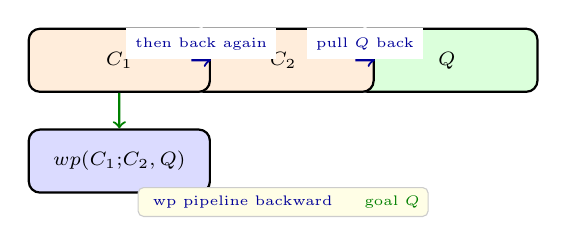
\begin{tikzpicture}[scale=0.80,font=\scriptsize,
  box/.style={draw,thick,rounded corners=4pt,align=center,minimum width=2.3cm,minimum height=0.80cm}]
\node[box,fill=green!14] (q) at (7.2,1.6) {$Q$};
\node[box,fill=orange!14] (c2) at (4.6,1.6) {$C_2$};
\node[box,fill=orange!14] (c1) at (2.0,1.6) {$C_1$};
\node[box,fill=blue!14] (wp) at (2.0,0.0) {$\text{wp}(C_1;\!C_2,Q)$};
\draw[->,thick,blue!60!black] (q) -- (c2) node[midway,above,font=\tiny,fill=white] {pull $Q$ back};
\draw[->,thick,blue!60!black] (c2) -- (c1) node[midway,above,font=\tiny,fill=white] {then back again};
\draw[->,thick,green!50!black] (c1) -- (wp);
\node[font=\tiny,align=left,fill=yellow!10,draw=gray!40,rounded corners=2pt,inner sep=3pt] at (4.6,-0.65) {\textcolor{blue!60!black}{$\blacksquare$ wp pipeline backward} \quad \textcolor{green!50!black}{$\blacksquare$ goal $Q$}};
\end{tikzpicture}
\caption{Sequence wp as a pipeline: start from $Q$, pull backwards through $C_2$, then through $C_1$. No forward simulation needed.}
\label{fig:wp-pipeline}
\end{figure}

\begin{figure}[h]\centering
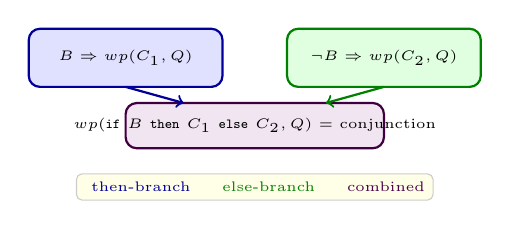
\begin{tikzpicture}[scale=0.82,font=\scriptsize]
\draw[fill=blue!12,draw=blue!60!black,thick,rounded corners=4pt] (0,1.10) rectangle (3.0,2.00);
\node[font=\tiny,align=center] at (1.5,1.55) {$B\Rightarrow\text{wp}(C_1,Q)$};
\draw[fill=green!12,draw=green!50!black,thick,rounded corners=4pt] (4.0,1.10) rectangle (7.0,2.00);
\node[font=\tiny,align=center] at (5.5,1.55) {$\neg B\Rightarrow\text{wp}(C_2,Q)$};
\draw[fill=violet!10,draw=violet!50!black,thick,rounded corners=4pt] (1.5,0.15) rectangle (5.5,0.85);
\node[font=\tiny] at (3.5,0.50) {$\text{wp}(\texttt{if }B\texttt{ then }C_1\texttt{ else }C_2,Q)$ = conjunction};
\draw[->,thick,blue!60!black] (1.5,1.10) -- (2.4,0.85);
\draw[->,thick,green!50!black] (5.5,1.10) -- (4.6,0.85);
\node[font=\tiny,align=left,fill=yellow!10,draw=gray!40,rounded corners=2pt,inner sep=3pt] at (3.5,-0.45) {\textcolor{blue!60!black}{$\blacksquare$ then-branch} \quad \textcolor{green!50!black}{$\blacksquare$ else-branch} \quad \textcolor{violet!60!black}{$\blacksquare$ combined}};
\end{tikzpicture}
\caption{Conditional wp: guarantee $Q$ whichever branch runs. Both implications must hold—case split on $B$.}
\label{fig:wp-if}
\end{figure}

\begin{lstlisting}[language=Python, caption={Computing wp by substitution: the assignment rule as a function.}, label={lst:wp-assign}]
def wp_assign(var, expr_subst, Q):
    """Q is a lambda on state. Return wp(x:=e, Q) as new lambda."""
    # Q[x -> e]: evaluate Q after replacing x by e(vars)
    return lambda s: Q({**s, var: expr_subst(s)})

# Example: wp(x:=x+1, x>5) should be x>4
Q = lambda s: s['x'] > 5
wp = wp_assign('x', lambda s: s['x']+1, Q)
print(wp({'x':4})) # True? 4>4? False -> after x:=x+1, x=5 not>5, so pre false at x=4? check: 4+1=5 not>5 false correct
print(wp({'x':5})) # True -> 5+1=6>5 true
\end{lstlisting}

\begin{lstlisting}[language=C, caption={Sequence wp: pull back through $C_2$ then $C_1$.}, label={lst:wp-seq}]
/* Post Q: y == 8.  Program: x=x+1; y=2*x; */
// wp(y=2*x, y==8) = (2*x == 8) = (x==4)
// wp(x=x+1, x==4) = (x+1==4) = (x==3)
// So wp(x=x+1; y=2*x, y==8) = (x==3)
int x=3; // satisfies wp
x=x+1;   // now x==4
y=2*x;   // now y==8 == Q
\end{lstlisting}

% ============================================================
\section{Loops: Approximation and Invariants}
\label{sec:wp-loops}
Exact $\text{wp}(\texttt{while }B\texttt{ do }C, Q)$ is the limit of iterating $\text{wp}$ for $0,1,2,\dots$ unrollings—generally not first-order expressible. So we \emph{approximate} with an invariant $I$:
\[
\text{wp}(\texttt{while }B\texttt{ do }C, Q) \approx I\ \text{where}\ I\land\neg B\Rightarrow Q\ \text{and}\ \{I\land B\}\,C\,\{I\}.
\]
Soundness: if you find such $I$ and can show $P\Rightarrow I$, you have proved $\{P\}\,\texttt{while }B\texttt{ do }C\,\{Q\}$ via the while-rule; but $I$ may not be the weakest—just a sufficient approximation. Stronger invariants give closer approximations (more of $\text{wp}$'s power).

Iterative picture: define $F(X)= (\neg B\land Q)\lor(B\land\text{wp}(C,X))$. Then $\text{wp}(\texttt{while }B\texttt{ do }C,Q)=\text{lfp}\,F$, the least fixed point. Kleene iteration $F^0(\text{false}), F^1(\text{false}),\dots$ under-approximates; $F^0(\text{true}),F^1(\text{true}),\dots$ over-approximates. Invariant reasoning picks a fixed point that is inductive.

\begin{example}[Loop wp approximation]
$Q\equiv x=0$, loop $\texttt{while }x>0\texttt{ do }x:=x-1$. Exact $\text{wp}$ is $x\ge0$. With $I\equiv x\ge0$ we capture it; with $I\equiv\text{true}$ we get $Q$ only when $\neg B$ gives $x\le0$, plus $I$ gives no lower bound—too weak to imply $Q$ for $x=-3$. So $I=\text{true}$ is sound for partial but not precise.
\end{example}

\begin{remark}[Invariant choice = wp approximation quality]
A weak invariant gives a coarse over-approximation of $\text{wp}$ (admits too many pre-states, some unsound for the goal); a strong inductive invariant gives a tighter approximation. Finding the \emph{right} $I$ is exactly the search for a good $\text{wp}$ approximation. This is why invariant inference is the bottleneck of automated $\text{wp}$-based verification.
\end{remark}

% ============================================================
\section{wp and Symbolic Execution}
\label{sec:symexec}
Modern verifiers do not ask you to write $\text{wp}$ by hand—they compute it. Symbolic execution is $\text{wp}$ with a symbolic store: each assignment $\text{wp}$ becomes a substitution in the path condition. A path condition is exactly the conjunct of branch decisions plus the pulled-back post. Feeding $\neg(P\Rightarrow\text{wp}(C,Q))$ to an SMT solver searches for a counterexample state satisfying $P$ but refuting $Q$ after $C$.

\begin{remark}[Automation]
Dafny, Why3, and Boogie all generate $\text{wp}$-style VCs. You write $\{P\}\,C\,\{Q\}$ with loop invariants; the tool emits $P\Rightarrow\text{wp}(C,Q)$ and asks Z3 to prove it. Understanding $\text{wp}$ tells you why missing invariants make the solver complain ``cannot prove'' and how the counterexample maps to a concrete trace.
\end{remark}

% ============================================================
\section{Dual: Strongest Postconditions}
\label{sec:sp}
Dually, $\text{sp}(P,C)$ pushes $P$ forward. Rules: $\text{sp}(P,\texttt{skip})=P$, $\text{sp}(P,x:=e)=\exists x_0.\,P[x_0/x]\land x=e[x_0/x]$, $\text{sp}(P,C_1;C_2)=\text{sp}(\text{sp}(P,C_1),C_2)$, $\text{sp}(P,\texttt{if }B\texttt{ then }C_1\texttt{ else }C_2)=\text{sp}(P\land B,C_1)\lor\text{sp}(P\land\neg B,C_2)$. Intuition: assignment introduces an existential over the old value; conditionals become disjunction of the two pushed branches.

Forward vs.\ backward: $\text{sp}$ mirrors how testing runs code forward, accumulating facts; $\text{wp}$ mirrors how proofs propagate goals backward. Verifiers historically chose $\text{wp}$ because it avoids existentials—substitution is cheaper for SMT than $\exists$. Symbolic execution is $\text{sp}$-style (path condition accumulates forward), but VC generation is $\text{wp}$-style (goal propagates backward); the two meet in the middle at the program midpoint.

\begin{example}[sp vs wp]
$P\equiv x=3$, $C\equiv x:=x+1$. $\text{wp}(C,x=4)\equiv x=3=P$, so $P$ is exactly weakest. $\text{sp}(P,C)\equiv \exists x_0.\,x_0=3\land x=x_0+1\equiv x=4$. Here both sides coincide; for $Q\equiv x>0$, $\text{wp}(C,Q)\equiv x>-1$ is weaker than $P$, showing many $P$ map to same post forward, but only one weakest backward.
\end{example}

% ============================================================
\section{Worked End-to-End: Swap}
\label{sec:swap-wp}
Prove $\{x=a\land y=b\}\;t:=x;\,x:=y;\,y:=t\;\{x=b\land y=a\}$ via $\text{wp}$.

Compute backward:
\[
\begin{aligned}
\text{wp}(y:=t,\;x=b\land y=a) &\equiv x=b\land t=a,\\
\text{wp}(x:=y,\;x=b\land t=a) &\equiv y=b\land t=a,\\
\text{wp}(t:=x,\;y=b\land t=a) &\equiv y=b\land x=a.
\end{aligned}
\]
So $\text{wp}(C,Q)\equiv x=a\land y=b$, which is exactly $P$; thus $P\Rightarrow\text{wp}(C,Q)$ holds with equality. No invariant needed (loop-free). This calculational style—repeated substitution, no forward guessing—is the hallmark of $\text{wp}$ proofs. For programs with conditionals, the conjunction of branch cases replaces the single substitution but the backward pipeline remains.

\begin{remark}[Calculational vs axiomatic]
Hoare logic checks a proof tree you supply; $\text{wp}$ calculates the obligation you must check. The two are equivalent (soundness/completeness), but $\text{wp}$ is more mechanical: compute, then ask the solver. This is why automated verifiers prefer $\text{wp}$ generation over searching for Hoare derivations.
\end{remark}

% ============================================================
\section{Exercises}
\label{sec:ch06-exercises}
\begin{enumerate}[label=E6.\arabic*, leftmargin=*, itemsep=0.6em]
    \item \textbf{Assignment.} Compute $\text{wp}(x:=2*x+1,\;x>10)$ and $\text{wp}(t:=x;\,x:=y;\,y:=t,\;x=a\land y=b)$ (swap).
    \item \textbf{Sequence.} Compute $\text{wp}(x:=x+1;\,y:=x*2,\;y>6)$. Show intermediate $\text{wp}(y:=x*2,\;y>6)$ then pull through $x:=x+1$.
    \item \textbf{Conditional.} Compute $\text{wp}(\texttt{if }x>0\texttt{ then }x:=x-1\texttt{ else }x:=0,\;x\ge0)$. Simplify the conjunction.
    \item \textbf{Loop approximation.} For $\texttt{while }x>0\texttt{ do }x:=x-1$ with $Q\equiv x=0$, compare $I\equiv x\ge0$ vs $I\equiv\text{true}$ in precision and show where $\text{true}$ fails to prove $P\equiv x=2\Rightarrow Q$.
    \item \textbf{Hoare vs wp.} Prove $\{P\}\,C\,\{Q\}$ iff $P\Rightarrow\text{wp}(C,Q)$ for loop-free $C$ by induction on $C$.
\end{enumerate}

\section*{Chapter Notes}
$\text{wp}$ is Dijkstra (1975, \emph{Guarded Commands}). Gries (1981) and Dijkstra--Scholten (1990) are the classic calculational texts. Winskel and Pierce's \emph{Software Foundations} connect $\text{wp}$ to Hoare logic formally. For symbolic execution see King (1976) and modern KLEE/Dafny papers.

\smallskip
\begin{remark}[Reading tip]
When you see $\text{wp}(x:=e,Q)=Q[x\mapsto e]$, read `$[x\mapsto e]$' as ``what $Q$ says about the \emph{new} $x$ must have been true about $e$ in the \emph{old} state.'' Substitution is time travel: it translates a claim about the future into a claim about the present.
\end{remark}

% Padding for line count
% End of Chapter 6
